\subsubsection{Uroflowmetry Base Plates}

The drawings below outline base plates fit for purpose, two are required. The large flat bottom provides a large stable base in contact with the floor as well as a large pad to place the fluid container on. 
The design centres the loadcell in the middle of the plate so that the weight of the container and fluid are over the centre of the plate. This reduces the likelihood of the container falling over if knocked.

\begin{figure}[h]
    \centering
    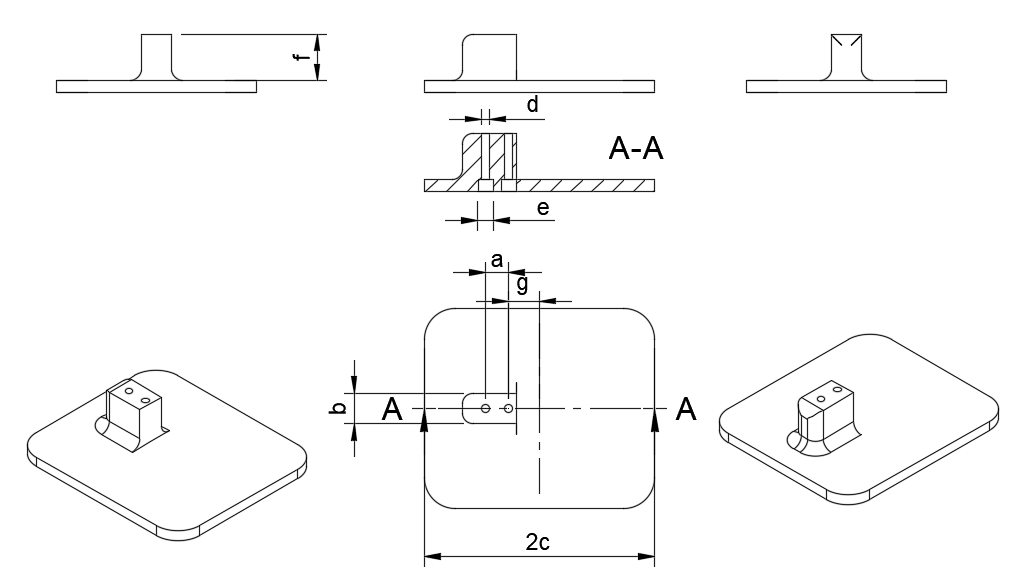
\includegraphics[width=0.7\textwidth]{Figures/SupportDrawings/uf_base_plate_drawing.png}
    \caption{Uroflowmetry Base Plate Drawings}
    \label{fig:ufbaseplatedrawing}
  \end{figure}

  \begin{enumerate}
    \item[a)] The distance between the centre points of the two tapped holes at each end of the loadcell
    \item[b)] The width of the loadcell + \textgreater\ 2mm
    \item[c)] Length of the loadcell
    \item[d)] The bolt diameter used by the loadcell + \textgreater\ 1mm
    \item[e)] The diameter of the head of the bolt + \textgreater\ 2mm 
    \item[f)] The height of the loadcell
    \item[g)] Distance between the centre of the loadcell and the centre point of the loadcell hole nearer to the loadcell mid-point
  \end{enumerate}